\documentclass[../../main.tex]{subfiles}
\begin{document}

\begin{flushright}
  \footnotesize\textit{【自動文字起こし・要確認】}
\end{flushright}

% Source: handwritten.pdf 第2問．
{\bf [解]}
\begin{align}0<x,y,\qquad y\ne x.\label{eq:1}
\end{align}
$b_n=\dfrac{a_n}{y^n}$によって$\{b_n\}$を定めると，$b_1=0$で，
\begin{align}b_{n+1}=\dfrac{x}{y}b_n+1.
\end{align}
\cref{eq:1}から
\begin{align}
  b_{n+1}-\dfrac{y}{y-x}=\dfrac{x}{y}\left(b_n-\dfrac{y}{y-x}\right).
\end{align}
くり返し用いて
\begin{align}
  b_n=\left(\dfrac{x}{y}\right)^{n-1}\left(-\dfrac{y}{y-x}\right)+\dfrac{y}{y-x},
\end{align}
\begin{align}
  a_n=\dfrac{y}{y-x}\left(y^n-x^{n-1}y\right)
  =\dfrac{y^2}{y-x}\left(y^{n-1}-x^{n-1}\right).
\end{align}
これが収束する条件は，\cref{eq:1}から，$y^{n-1}-x^{n-1}$が収束する条件と等しい．
\subparagraph{(i) $y>x>0$のとき}
\begin{align}
  y^{n-1}-x^{n-1}=y^{n-1}\left\{1-\left(\dfrac{x}{y}\right)^{n-1}\right\}
\end{align}
が収束するには，$0<y\leqq1$が条件である．
\subparagraph{(ii) $x>y>0$のとき}
同じく，$0<x\leqq1$が条件である．
\casesend
以上まとめて
\begin{align}0<x<y\leqq1\quad\text{又は}\quad0<y<x\leqq1.
\end{align}
だから，図示して図の着色部．境界は$x=1$，$y=1$は含み，$x=0$，$y=0$は含まず，$y=x$は含まない．
\begin{figure}[H]
  \centering
  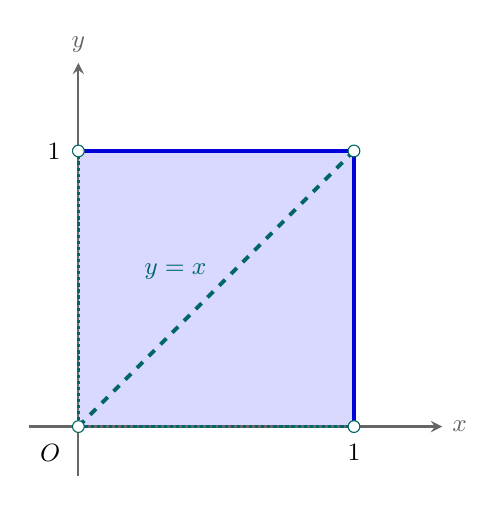
\begin{tikzpicture}[x=3.5cm, y=3.5cm, >=stealth,
    every node/.style={font=\small}]
    \fill[blue!15] (0,0) rectangle (1,1);
    \draw[->, thick, gray!80!black] (-0.18,0) -- (1.32,0) node[right] {$x$};
    \draw[->, thick, gray!80!black] (0,-0.18) -- (0,1.32) node[above] {$y$};
    \draw[line width=1.4pt, blue!85!black] (0,1) -- (1,1) -- (1,0);
    \draw[dashed, line width=1.4pt, teal!80!black] (0,0) -- (1,1);
    \draw[densely dotted, line width=1.2pt, teal!80!black]
    (0,0) -- (1,0) (0,0) -- (0,1);
    \foreach \x/\y in {0/0,1/0,0/1,1/1}
    \node[circle, draw, teal!80!black, fill=white, inner sep=1.5pt] at (\x,\y) {};
    \node[below left=3pt] at (0,0) {$O$};
    \node[below=3pt] at (1,0) {$1$};
    \node[left=3pt] at (0,1) {$1$};
    \node[teal!80!black, above left] at (0.5,0.5) {$y=x$};
  \end{tikzpicture}
  \caption{数列が有限の値に収束する$(x,y)$の範囲}
\end{figure}

\end{document}
